  \documentclass[final]{beamer} % beamer 3.10: do NOT use option hyperref={pdfpagelabels=false} !
% don't show navigation symbols
% 2016 A. Kleiber
% 2018 A. Kleiber
\beamertemplatenavigationsymbolsempty
  \usepackage{2018_10_beamerouterthemeposterasdex}
  \usepackage[english]{babel}
  \usepackage[latin1]{inputenc}
	\usepackage{tcolorbox}
  \usepackage{amsmath, amsthm, amssymb, latexsym, stackrel}
	% Arial-Schrift
  %\usepackage{ipp}
  %\usepackage[scaled]{uarial}
  %\usepackage{times}\usefonttheme{professionalfonts}  % times is obsolete
  %\usefonttheme[onlymath]{serif}
  \boldmath
  \usepackage[orientation=portrait,size=a0,scale=1.4,debug]{2018_10_beamerposteripp}                       % e.g. for DIN-A0 poster
  %\usepackage[orientation=portrait,size=a1,scale=1.4,grid,debug]{beamerposter}                  % e.g. for DIN-A1 poster, with optional grid and debug output
  %\usepackage[size=custom,width=200,height=120,scale=2,debug]{beamerposter}                     % e.g. for custom size poster
  %\usepackage[orientation=portrait,size=a0,scale=1.0,printer=rwth-glossy-uv.df]{beamerposter}   % e.g. for DIN-A0 poster with rwth-glossy-uv printer check
  % ...
  %
\setbeamertemplate{bibliography item}{\insertbiblabel}
% Damit im Literaturverzeichnis Zahlen stehen.

% title of the presentation
  \title{Title of presentation }
	% Sollte die Ueberschrift zu lang sein, kann sie wie folgt auf zwei Zeilen umgebrochen werden: 
	%\title{Effects of collisions on the saturation dynamics\linebreak \hspace*{6ex}
    %of TAEs in tokamaks and stellarators}
% authors of the presentation
  \author[Author]{A.~Author\inst{1}*, B.~Author\inst{2}, C.~Author\inst{3}}
% email address of the corresponding author 
% Definieren mail corresponding author
  \newcommand{\emailcorrespondingauthor}{A.author@ipp.mpg.de}
% Definieren Name Conference
  \newcommand{\nameconference}{Name der Konferenz Da.Tu.M000}
% institutes of the authors
%  \institute[IPP Greifswald]{\inst{1}Max Planck Institute for Plasma Physics, 
%                             Wendelsteinstr. 1, D-17491 Greifswald, Germany}
 \institute[]{%\hspace{5cm}
     \inst{1}Max Planck Institute for Plasma Physics, Boltzmannstr., D-85748 Garching, Germany, 
     \inst{2}Institute 2, street2, town2, country2, 
	 \inst{3}Institute 3, street3, town3, country3 
     } 
% name of the conference
 %\nameconference{Name der Konferenz Da.Tu.M000}
% set date of the talk
  \date{\today}
%%%%%%%%%%%%%%%%%%%%%%%%%%%%%%%%%%%%%%%%%%%%%%%%%%%%%%%%%%%%%%%%%%%%%%%% 
% 
%%%%%%%%%%%%%%%%%%%%%%%%%%%%%%%%%%%%%%%%%%%%%%%%%%%%%%%%%%%%%%%%%%%%%%%% 
  \begin{document}
  %\begin{frame}{}
  \begin{frame}
  \frametitle{}
%%%%%%%%%%%%%%%%%%%%%%%%%%%%%%%%%%%%%%%%%%%%%%%%%%%%%%%%%%%%%%%%%%%%%%%% 
% Text über beide Spalten
%%%%%%%%%%%%%%%%%%%%%%%%%%%%%%%%%%%%%%%%%%%%%%%%%%%%%%%%%%%%%%%%%%%%%%%% 
Es geht auch einfacher Text.
%%%%%%%%%%%%%%%%%%%%%%%%%%%%%%%%%%%%%%%%%%%%%%%%%%%%%%%%%%%%%%%%%%%%%%%% 
% Kasten über beide Spalten
%%%%%%%%%%%%%%%%%%%%%%%%%%%%%%%%%%%%%%%%%%%%%%%%%%%%%%%%%%%%%%%%%%%%%%%% 
    \begin{kasten}{\large Simple list}
      \begin{enumerate}
        \item item1
        \item item2
        \item item3
        \item item4
        \item item5
        \item item6
      \end{enumerate}
    \end{kasten}
%%%%%%%%%%%%%%%%%%%%%%%%%%%%%%%%%%%%%%%%%%%%%%%%%%%%%%%%%%%%%%%%%%%%%%%% 
% Kasten über beide Spalten
%%%%%%%%%%%%%%%%%%%%%%%%%%%%%%%%%%%%%%%%%%%%%%%%%%%%%%%%%%%%%%%%%%%%%%%% 
    \begin{kasten}{\large text and figure}
    \begin{columns}
    \column{.45\textwidth}
      \begin{enumerate}
        \item item1
        \item item2
        \item item3
        \item item4
        \item item5
        \item item6
      \end{enumerate}\hfill
    \column{.45\textwidth}
    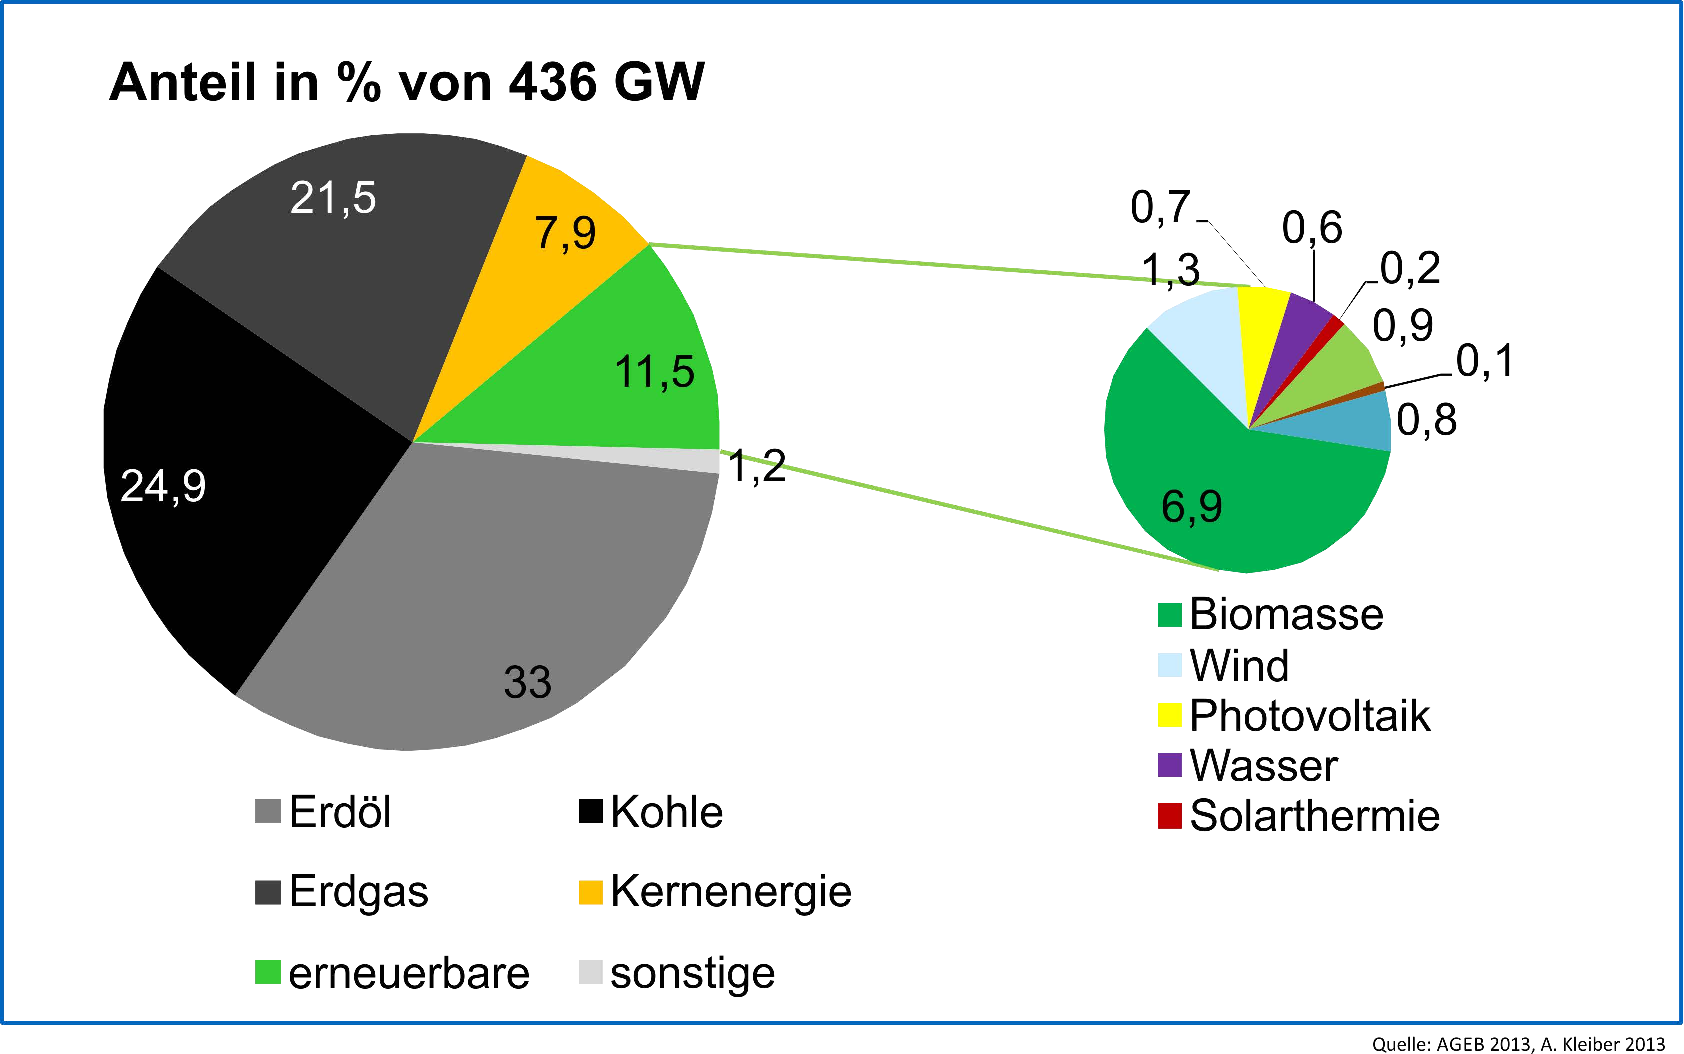
\includegraphics[width=.7\textwidth]{primaerenergieverbrauch_dt_2013}\par
    Figure caption.
    \end{columns}
    \end{kasten}
		
%%%%%%%%%%%%%%%%%%%%%%%%%%%%%%%%%%%%%%%%%%%%%%%%%%%%%%%%%%%%%%%%%%%%%%%% 
% linke Spalte
%%%%%%%%%%%%%%%%%%%%%%%%%%%%%%%%%%%%%%%%%%%%%%%%%%%%%%%%%%%%%%%%%%%%%%%% 
  \begin{minipage}[t]{.49\textwidth}
%%%%%%%%%%%%%%%%%%%%%%%%%%%%%%%%%%%%%%%%%%%%%%%%%%%%%%%%%%%%%%%%%%%%%%%% 
Ab jetzt geht es in Spalten weiter. Hier die linke Spalte.
%%%%%%%%%%%%%%%%%%%%%%%%%%%%%%%%%%%%%%%%%%%%%%%%%%%%%%%%%%%%%%%%%%%%%%%% 
    \begin{kasten}{\large list}
      \begin{itemize}
        \item new item1
        \item new item2
        \item new item3
        \item new item4
        \item new item5
        \item new item6
      \end{itemize}
    \end{kasten}
%%%%%%%%%%%%%%%%%%%%%%%%%%%%%%%%%%%%%%%%%%%%%%%%%%%%%%%%%%%%%%%%%%%%%%%% 
    \begin{kasten}{\large two blocks}
      %\setbeamercovered{transparent}
      \begin{kasten2}{block description}
        some text or formula $$\sum\limits_{i=1}^n i = \frac{n (n+1)}{2}$$
      \end{kasten2}
      \begin{kasten2}{block description 2}
        more notes {\tiny small notes}
      \end{kasten2}
    \end{kasten}
%%%%%%%%%%%%%%%%%%%%%%%%%%%%%%%%%%%%%%%%%%%%%%%%%%%%%%%%%%%%%%%%%%%%%%%%% 
    \begin{kasten}{\large two lists}
      \begin{itemize}
        \item important1 \cite{Feher13}
        \item important2
        \item important3
      \end{itemize}
      \begin{itemize}
        \item item1 \cite{Koenies12}
        \item item2
        \item item3
        \item item4
      \end{itemize}
    \end{kasten}
%%%%%%%%%%%%%%%%%%%%%%%%%%%%%%%%%%%%%%%%%%%%%%%%%%%%%%%%%%%%%%%%%%%%%%%% 
    \begin{kasten}{\large figures}
      \begin{center}
      \frametitle{figures}
      \begin{minipage}[]{0.45\textwidth}
        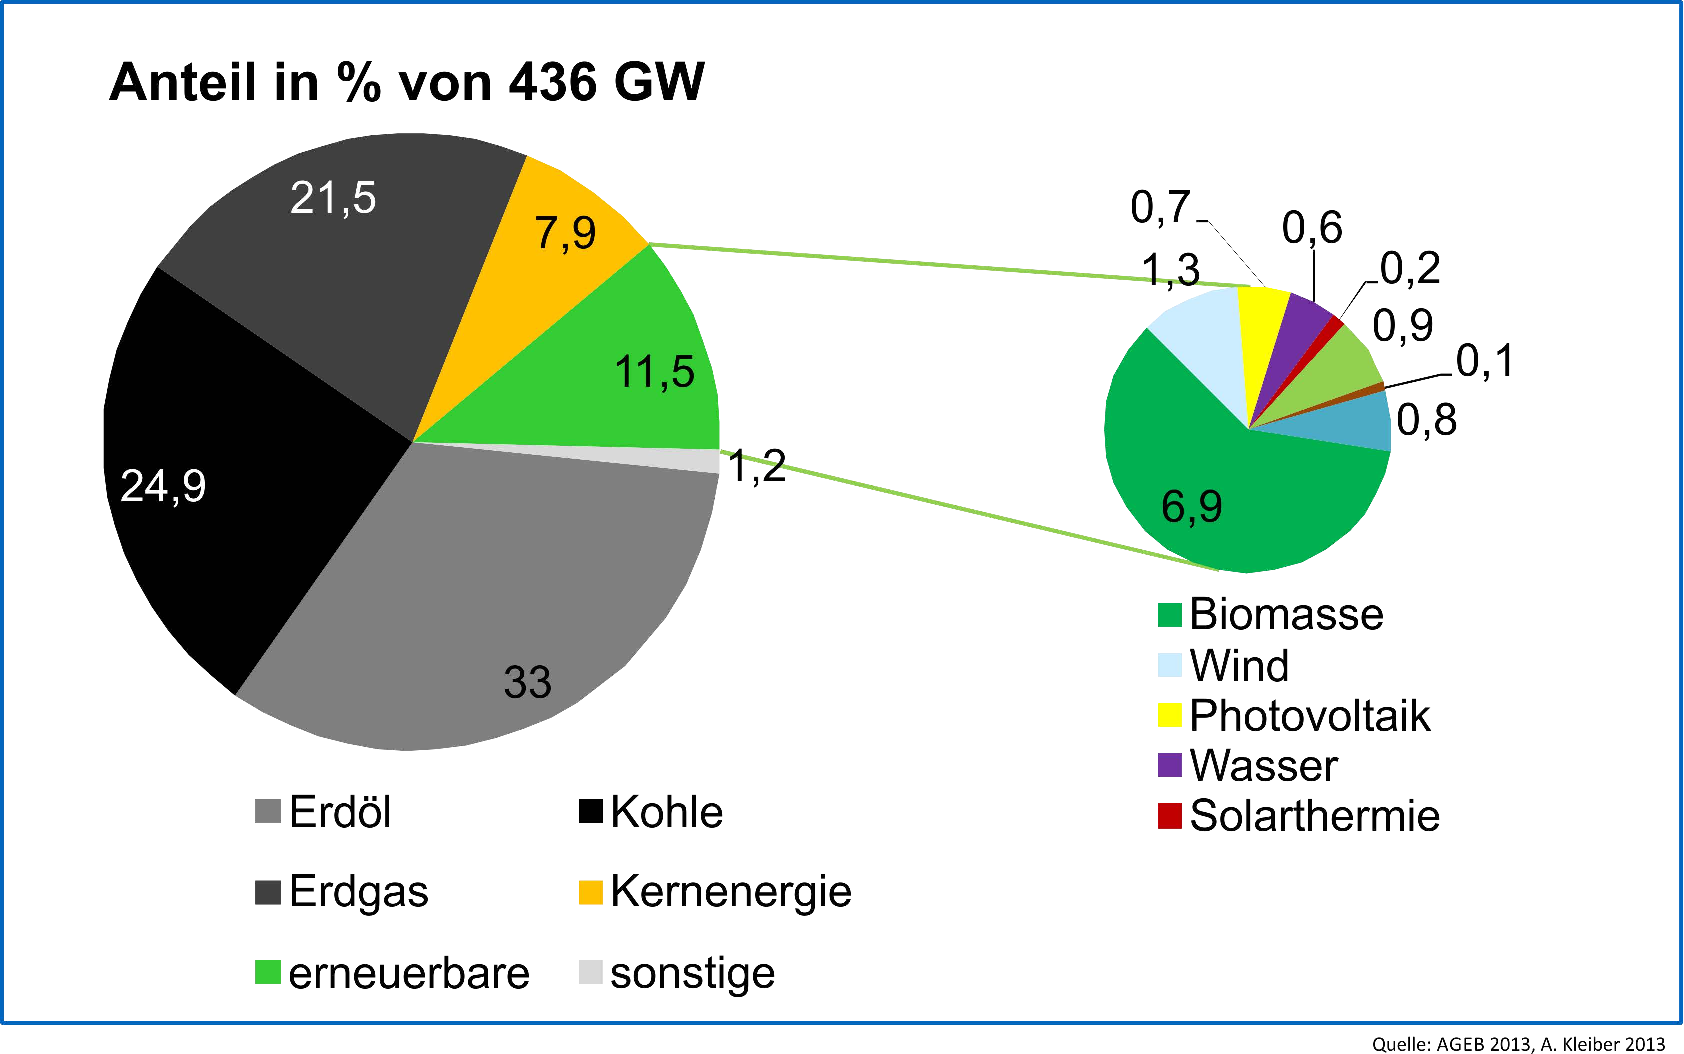
\includegraphics[width=\textwidth]{primaerenergieverbrauch_dt_2013}\par
        figure caption.
      \end{minipage}\hfill
      \begin{minipage}[]{0.45\textwidth}
			  \centerline{
        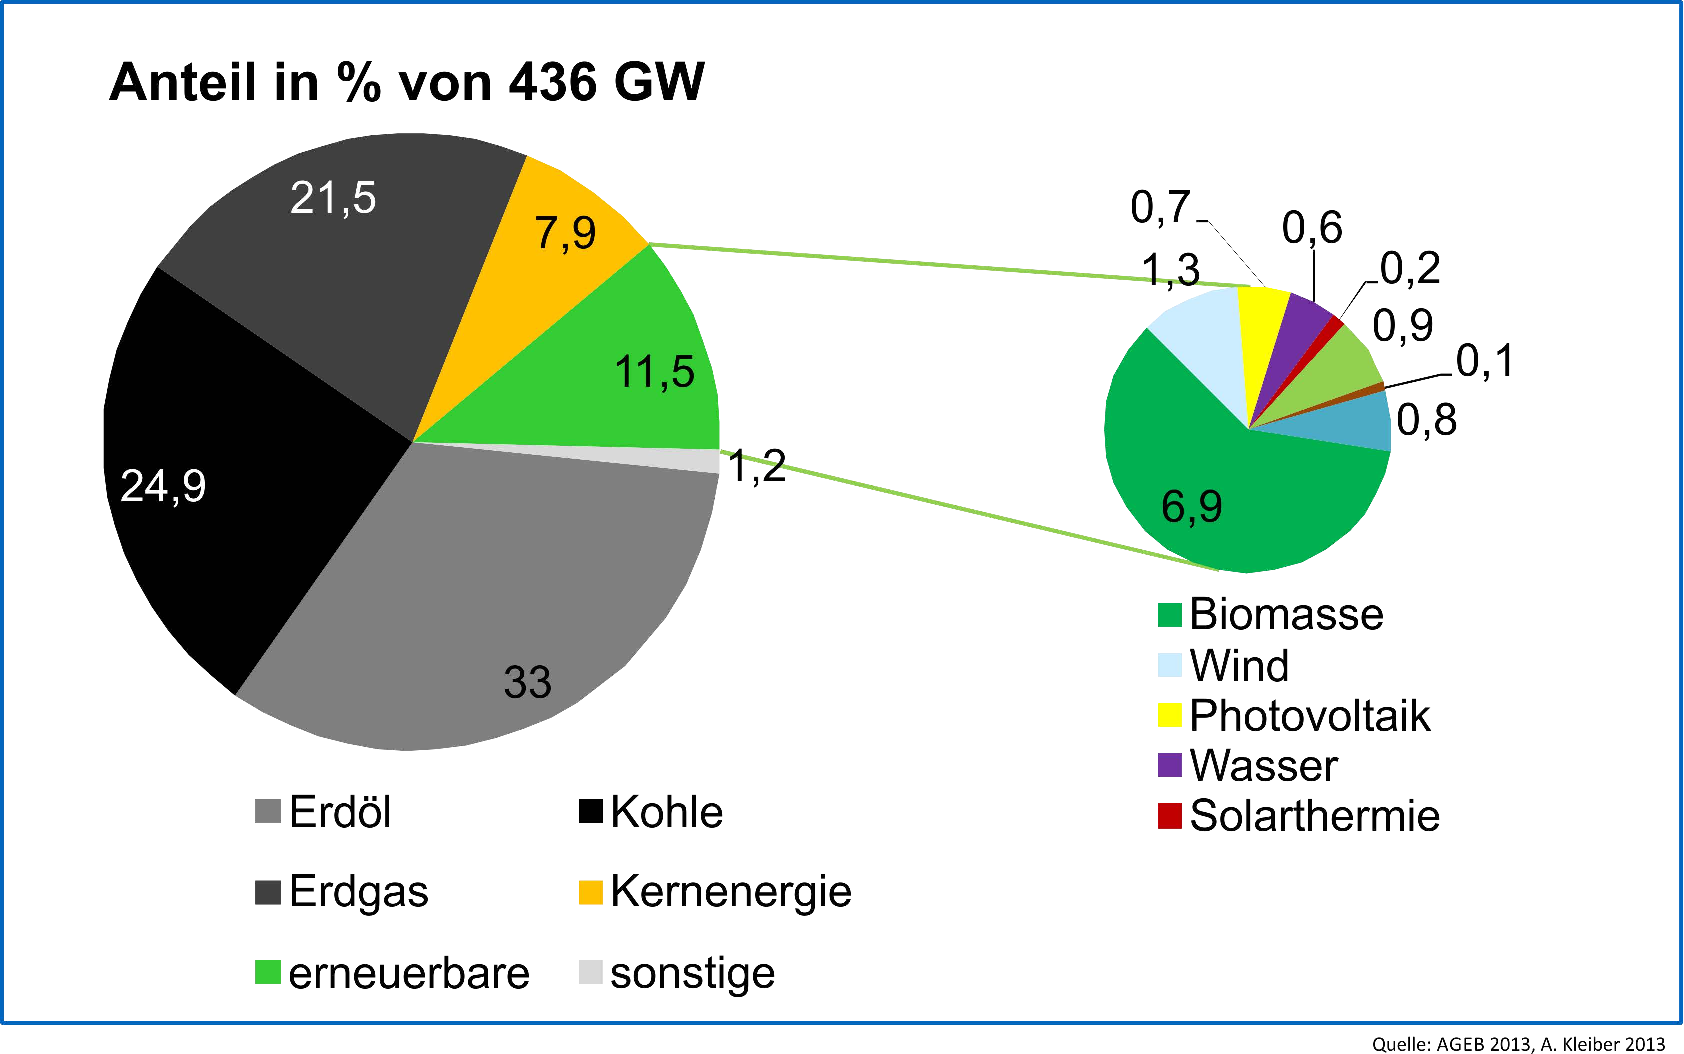
\includegraphics[width=.8\textwidth]{primaerenergieverbrauch_dt_2013}}\par
        figure caption 2.
      \end{minipage}
      \end{center}
    \end{kasten}
%%%%%%%%%%%%%%%%%%%%%%%%%%%%%%%%%%%%%%%%%%%%%%%%%%%%%%%%%%%%%%%%%%%%%%%%% 
  \vfill
  \end{minipage}\hfill
%%%%%%%%%%%%%%%%%%%%%%%%%%%%%%%%%%%%%%%%%%%%%%%%%%%%%%%%%%%%%%%%%%%%%%%%% 
%% rechte Spalte
%%%%%%%%%%%%%%%%%%%%%%%%%%%%%%%%%%%%%%%%%%%%%%%%%%%%%%%%%%%%%%%%%%%%%%%%% 
  \begin{minipage}[t]{.49\textwidth}
%%%%%%%%%%%%%%%%%%%%%%%%%%%%%%%%%%%%%%%%%%%%%%%%%%%%%%%%%%%%%%%%%%%%%%%%% 
Und dies ist der Beginn der rechten Spalte. Mit ein wenig Text.
%%%%%%%%%%%%%%%%%%%%%%%%%%%%%%%%%%%%%%%%%%%%%%%%%%%%%%%%%%%%%%%%%%%%%%%%% 
    \begin{kasten}{\large columns}
      \begin{columns}
        \column{6cm}
          some text on the left hand side
        \column{4cm}
          text for the right hand side
      \end{columns}
    \end{kasten}
%%%%%%%%%%%%%%%%%%%%%%%%%%%%%%%%%%%%%%%%%%%%%%%%%%%%%%%%%%%%%%%%%%%%%%%% 
    \begin{kasten}{\large text}
      text text text text text text text text text text text text text 
			text text text text text text text text text text text text text 
			text text text text text text text text text text text text text 
			text text text text text text text text text text text text text 
			text text text text text text text text text text text text text 
			text text text text text text text text text text text text text 
			text text text text text text text text text text text text text 
			text text text text text text text text text text text text text 
			text text text text text text text text text text text text text 
			text text text text text text text text text text text text text 
			text text text text text text text text text text text text text 
			text text text text text text text text text text text text text 
			text text text text text text text text text text text text text 
			text text text text text text text text text text text text text 
			text text text text text text text text text text text text text 
			text text text text text text text text text text text text text 
			text text text text text text text text text text text text text 
			text text text text text text text text text text text text text 
    \end{kasten}
		%%%%%%%%%%%%%%%%%%%%%%%%%%%%%%%%%%%%%%%%%%%%%%%%%%%%%%%%%%%%%%%%%%%%%%%%% 
    \begin{kasten}{\large two lists}
      \begin{itemize}
        \item important1
        \item important2
        \item important3
        \item important4
      \end{itemize}
      \begin{itemize}
        \item item1
        \item item2
      \end{itemize}
    \end{kasten}
%%%%%%%%%%%%%%%%%%%%%%%%%%%%%%%%%%%%%%%%%%%%%%%%%%%%%%%%%%%%%%%%%%%%%%%% 
    \begin{kasten}{\large References}
      \small
      \begin{thebibliography}{}
        \bibitem{Feher13} T. B. Feh\'er, Ph.D. thesis, University   Greifswald, 2013
        \bibitem{Koenies07} A. K\"onies \textit{et al.}, 10th IAEA TM on Energetic Particles in Magnetic Confinement Systems (Kloster Seeon, 2007)
        \bibitem{Slaby17} C. Slaby \textit{et al.}, Comp. Phys. Comm. \textbf{218}, 1-9 (2017)
        \bibitem{Koenies12} A. K\"onies \textit{et al.}, 24th IAEA Fusion Energy Conference (San Diego, 2012)
        \bibitem{Berk92} H. L. Berk \textit{et al.}, Phys. Rev. Lett. \textbf{68}, 3563 (1992)
      \end{thebibliography}
    \end{kasten}
%%%%%%%%%%%%%%%%%%%%%%%%%%%%%%%%%%%%%%%%%%%%%%%%%%%%%%%%%%%%%%%%%%%%%%%%% 
  \vfill
  \end{minipage}
%%%%%%%%%%%%%%%%%%%%%%%%%%%%%%%%%%%%%%%%%%%%%%%%%%%%%%%%%%%%%%%%%%%%%%%% 
  \end{frame}
\end{document}

